\documentclass[11pt,a4paper]{article}

\usepackage[margin=2.5cm]{geometry}
\usepackage{amsmath,amssymb,amsthm}
\usepackage{booktabs}
\usepackage{multirow}
\usepackage{colortbl}
\usepackage[table]{xcolor}
\usepackage{array}
\usepackage{graphicx}
\usepackage{float}
\usepackage{diagbox}
\usepackage{tikz}
\usetikzlibrary{arrows.meta,positioning,calc}
\usepackage{hyperref}
\usepackage{draftwatermark}
\SetWatermarkText{WORKING PAPER}
\SetWatermarkScale{1.5}
\SetWatermarkAngle{45}
\SetWatermarkColor[gray]{0.80}

% ---------------------------------------------------------------
% Theorem environments
% ---------------------------------------------------------------
\newtheorem{theorem}{Theorem}[section]
\newtheorem{lemma}[theorem]{Lemma}
\newtheorem{proposition}[theorem]{Proposition}
\newtheorem{corollary}[theorem]{Corollary}
\newtheorem{definition}[theorem]{Definition}
\theoremstyle{remark}
\newtheorem{example}[theorem]{Example}
\theoremstyle{plain}
\newtheorem{conjecture}[theorem]{Conjecture}
\newtheorem{remark}[theorem]{Remark}

% ---------------------------------------------------------------
% Global residue palette.
% Colour index = residue value (0..23), shared across all columns.
% Cell (n, c) gets colour res_{n mod c}.
% Since n mod c is the same for all c >= first_distinguishing_modulus(n),
% cells from that column rightward all share the same colour.
% Odd rows are coloured; even rows are white.
% 24 evenly-spaced pastel hues (HSL: saturation 0.6, lightness 0.85).
% ---------------------------------------------------------------
\definecolor{res0}{HTML}{EFC1C1}
\definecolor{res1}{HTML}{EFCDC1}
\definecolor{res2}{HTML}{EFD8C1}
\definecolor{res3}{HTML}{EFE4C1}
\definecolor{res4}{HTML}{EFEFC1}
\definecolor{res5}{HTML}{E4EFC1}
\definecolor{res6}{HTML}{D8EFC1}
\definecolor{res7}{HTML}{CDEFC1}
\definecolor{res8}{HTML}{C1EFC1}
\definecolor{res9}{HTML}{C1EFCD}
\definecolor{res10}{HTML}{C1EFD8}
\definecolor{res11}{HTML}{C1EFE4}
\definecolor{res12}{HTML}{C1EFEF}
\definecolor{res13}{HTML}{C1E4EF}
\definecolor{res14}{HTML}{C1D8EF}
\definecolor{res15}{HTML}{C1CDEF}
\definecolor{res16}{HTML}{C1C1EF}
\definecolor{res17}{HTML}{CDC1EF}
\definecolor{res18}{HTML}{D8C1EF}
\definecolor{res19}{HTML}{E4C1EF}
\definecolor{res20}{HTML}{EFC1EF}
\definecolor{res21}{HTML}{EFC1E4}
\definecolor{res22}{HTML}{EFC1D8}
\definecolor{res23}{HTML}{EFC1CD}

% Greyscale palette for magnitude columns (g0=white, g23=medium grey)
% 24 steps from #FFFFFF down to #AAAAAA
\definecolor{g0}{HTML}{FFFFFF}
\definecolor{g1}{HTML}{FCFCFC}
\definecolor{g2}{HTML}{F9F9F9}
\definecolor{g3}{HTML}{F6F6F6}
\definecolor{g4}{HTML}{F3F3F3}
\definecolor{g5}{HTML}{F0F0F0}
\definecolor{g6}{HTML}{EDEDED}
\definecolor{g7}{HTML}{EAEAEA}
\definecolor{g8}{HTML}{E7E7E7}
\definecolor{g9}{HTML}{E4E4E4}
\definecolor{g10}{HTML}{E1E1E1}
\definecolor{g11}{HTML}{DEDEDE}
\definecolor{g12}{HTML}{DBDBDB}
\definecolor{g13}{HTML}{D8D8D8}
\definecolor{g14}{HTML}{D5D5D5}
\definecolor{g15}{HTML}{D2D2D2}
\definecolor{g16}{HTML}{CFCFCF}
\definecolor{g17}{HTML}{CCCCCC}
\definecolor{g18}{HTML}{C9C9C9}
\definecolor{g19}{HTML}{C6C6C6}
\definecolor{g20}{HTML}{C3C3C3}
\definecolor{g21}{HTML}{C0C0C0}
\definecolor{g22}{HTML}{BCBCBC}
\definecolor{g23}{HTML}{AAAAAA}

% ---------------------------------------------------------------

\title{A Regular Expression Language for the Collatz Graph}
\author{Jon Seymour\\
  \texttt{jon@wildducktheories.com}\\
  Sydney, Australia}
\date{July 2026}

\begin{document}

\maketitle

\begin{abstract}
The Syracuse map $S(n) = (3n+1)/2^{v_2(3n+1)}$ partitions every orbit into
\emph{Steiner circuits}: maximal runs of the form $(\text{OE})^*\,\text{OEE}^+$,
where each step is classified by the 2-adic valuation $v = v_2(3n+1)$ and
equivalently by the residue of the input $n \bmod 8$.
The residue alphabet $\{1, 3, 5, 7\}$ encodes the four step types:
OE steps ($v = 1$, $n \equiv 3$ or $7 \bmod 8$),
OEE steps ($v = 2$, $n \equiv 1 \bmod 8$), and
OEEE$^+$ steps ($v \geq 3$, $n \equiv 5 \bmod 8$).
Within this alphabet, every Steiner circuit is conjectured to match the regular
expression $(7^*3)?(1|5)$ and every complete Collatz orbit to match $((7^*3)?(1|5))^*$.
This paper develops the combinatorial infrastructure supporting these conjectures:
the mod-8 step taxonomy, the Steiner circuit decomposition (proved), the 7-run
length theorem (proved), and the \emph{mod-24 universe} --- the smallest modular
arena in which the parity prefix of every odd residue class is fully determined
(established by explicit enumeration).
The regular-expression characterisation itself is stated as a conjecture; its proof
is deferred to the companion paper~\cite{paper5}.
Further analytic tools and cycle-theoretic consequences are developed
in the companion papers~\cite{paper5,paper8}.

\medskip
\noindent\textbf{Status.}
This is a working paper.
All theorems carry complete proofs.
Results labelled \emph{Conjecture} are stated precisely but not yet proved.
Deferred material is clearly flagged.
\end{abstract}

\tableofcontents

\section*{Note on paper numbering}

This paper is Paper~1 in a four-paper series.
Papers are numbered by their mod-8 significance:
Paper~1 (architecture), Paper~5 (tools), Paper~8 (results), Paper~0 (capstone).
On the filesystem the series lives under \texttt{papers/\{32+p\}-\{slug\}/}.

\bigskip\hrule\bigskip

%% Sections to be written %%

\section{Introduction}

% ---------------------------------------------------------------
% Chapter 1: discursive introduction.
% Describe the architecture of the paper, defer graphs and regular
% expressions to later chapters. To be written.
% ---------------------------------------------------------------

\subsection{The Collatz Maps}

Let $\mathbb{Z}^+ = \{1, 2, 3, \ldots\}$ be the positive integers,
$\mathbb{O} = \{n \in \mathbb{Z}^+ : n \text{ odd}\}$ the positive odd integers, and
$v_2(m)$ the 2-adic valuation of $m$ (the largest power of~$2$ dividing~$m$).

\begin{definition}[Natural, Syracuse, and Terras maps]\label{def:maps}
The \emph{natural Collatz map} $C : \mathbb{Z}^+ \to \mathbb{Z}^+$ is defined by
\[
  C(n) \;=\; \begin{cases} n/2 & \text{if } n \text{ is even,} \\ 3n+1 & \text{if } n \text{ is odd.} \end{cases}
\]
The \emph{Syracuse map} $S : \mathbb{O} \to \mathbb{O}$ is obtained by collapsing
every run of even steps into a single transition:
\[
  S(n) \;=\; \frac{3n+1}{2^{v_2(3n+1)}}, \qquad n \in \mathbb{O}.
\]
Every orbit of $C$ visits $\mathbb{O}$ after at most finitely many even steps, so $S$
records exactly the odd nodes visited by $C$, with even intermediates suppressed.
The two maps are related by $S(n) = C^{v_2(3n+1)+1}(n)$ for all $n \in \mathbb{O}$.

The \emph{Terras map} $T : \mathbb{Z}^+ \to \mathbb{Z}^+$~\cite{terras1976} is defined by
\[
  T(n) \;=\; \begin{cases} n/2 & \text{if } n \text{ is even,} \\ (3n+1)/2 & \text{if } n \text{ is odd.} \end{cases}
\]
Note that $T(n)$ is not generally odd when $n$ is odd; the Terras map steps from odd integer to
integer (odd or even), whereas $S$ steps from odd integer to odd integer.
Note that $T$ maps odd inputs to integers that may themselves be even, so iterating
$T$ does not in general recover $S$.
The correct relation between $S$ and $C$ is $S(n) = C^{v_2(3n+1)+1}(n)$ for all
$n \in \mathbb{O}$: one application of $C$ to the odd input $n$ produces $3n+1$,
and $v_2(3n+1)$ further applications of $C$ perform the mandatory halvings.
\end{definition}

% ---------------------------------------------------------------
\section{The Mod-24 Universe}
\label{sec:mod24}

\subsection{Residue Table}

Every odd integer $a$ belongs to one of twelve odd residue classes modulo~24.
The table below records $a \bmod c$ for each $c \in \{2,3,4,6,8,12,16,24\}$
and each representative $a \in \{0,1,\ldots,23\}$.
Even rows are white; odd rows are coloured by a single global palette in which
colour index equals residue value.
Because $a \bmod c = a \bmod c'$ for all $c' \geq c$ once $c$ first resolves $a$,
each odd row's colour is constant from the first resolving column rightward,
making the coarsening hierarchy visible at a glance.

\vspace{1em}
\noindent
\begin{tabular}{>{\bfseries}r|rrrrrrrr}
\toprule
$a$ & $\bmod 2$ & $\bmod 3$ & $\bmod 4$ & $\bmod 6$ & $\bmod 8$ & $\bmod 12$ & $\bmod 16$ & $\bmod 24$ \\
\midrule
  \textbf{0} & 0 & 0 & 0 & 0 & 0 & 0 & 0 & 0 \\
  \textbf{1} & \cellcolor{res1}1 & \cellcolor{res1}1 & \cellcolor{res1}1 & \cellcolor{res1}1 & \cellcolor{res1}1 & \cellcolor{res1}1 & \cellcolor{res1}1 & \cellcolor{res1}1 \\
  \hline
  \textbf{2} & 0 & 2 & 2 & 2 & 2 & 2 & 2 & 2 \\
  \textbf{3} & \cellcolor{res1}1 & \cellcolor{res0}0 & \cellcolor{res3}3 & \cellcolor{res3}3 & \cellcolor{res3}3 & \cellcolor{res3}3 & \cellcolor{res3}3 & \cellcolor{res3}3 \\
  \hline
  \textbf{4} & 0 & 1 & 0 & 4 & 4 & 4 & 4 & 4 \\
  \textbf{5} & \cellcolor{res1}1 & \cellcolor{res2}2 & \cellcolor{res1}1 & \cellcolor{res5}5 & \cellcolor{res5}5 & \cellcolor{res5}5 & \cellcolor{res5}5 & \cellcolor{res5}5 \\
  \hline
  \textbf{6} & 0 & 0 & 2 & 0 & 6 & 6 & 6 & 6 \\
  \textbf{7} & \cellcolor{res1}1 & \cellcolor{res1}1 & \cellcolor{res3}3 & \cellcolor{res1}1 & \cellcolor{res7}7 & \cellcolor{res7}7 & \cellcolor{res7}7 & \cellcolor{res7}7 \\
  \hline
  \textbf{8} & 0 & 2 & 0 & 2 & 0 & 8 & 8 & 8 \\
  \textbf{9} & \cellcolor{res1}1 & \cellcolor{res0}0 & \cellcolor{res1}1 & \cellcolor{res3}3 & \cellcolor{res1}1 & \cellcolor{res9}9 & \cellcolor{res9}9 & \cellcolor{res9}9 \\
  \hline
  \textbf{10} & 0 & 1 & 2 & 4 & 2 & 10 & 10 & 10 \\
  \textbf{11} & \cellcolor{res1}1 & \cellcolor{res2}2 & \cellcolor{res3}3 & \cellcolor{res5}5 & \cellcolor{res3}3 & \cellcolor{res11}11 & \cellcolor{res11}11 & \cellcolor{res11}11 \\
  \hline
  \textbf{12} & 0 & 0 & 0 & 0 & 4 & 0 & 12 & 12 \\
  \textbf{13} & \cellcolor{res1}1 & \cellcolor{res1}1 & \cellcolor{res1}1 & \cellcolor{res1}1 & \cellcolor{res5}5 & \cellcolor{res1}1 & \cellcolor{res13}13 & \cellcolor{res13}13 \\
  \hline
  \textbf{14} & 0 & 2 & 2 & 2 & 6 & 2 & 14 & 14 \\
  \textbf{15} & \cellcolor{res1}1 & \cellcolor{res0}0 & \cellcolor{res3}3 & \cellcolor{res3}3 & \cellcolor{res7}7 & \cellcolor{res3}3 & \cellcolor{res15}15 & \cellcolor{res15}15 \\
  \hline
  \textbf{16} & 0 & 1 & 0 & 4 & 0 & 4 & 0 & 16 \\
  \textbf{17} & \cellcolor{res1}1 & \cellcolor{res2}2 & \cellcolor{res1}1 & \cellcolor{res5}5 & \cellcolor{res1}1 & \cellcolor{res5}5 & \cellcolor{res1}1 & \cellcolor{res17}17 \\
  \hline
  \textbf{18} & 0 & 0 & 2 & 0 & 2 & 6 & 2 & 18 \\
  \textbf{19} & \cellcolor{res1}1 & \cellcolor{res1}1 & \cellcolor{res3}3 & \cellcolor{res1}1 & \cellcolor{res3}3 & \cellcolor{res7}7 & \cellcolor{res3}3 & \cellcolor{res19}19 \\
  \hline
  \textbf{20} & 0 & 2 & 0 & 2 & 4 & 8 & 4 & 20 \\
  \textbf{21} & \cellcolor{res1}1 & \cellcolor{res0}0 & \cellcolor{res1}1 & \cellcolor{res3}3 & \cellcolor{res5}5 & \cellcolor{res9}9 & \cellcolor{res5}5 & \cellcolor{res21}21 \\
  \hline
  \textbf{22} & 0 & 1 & 2 & 4 & 6 & 10 & 6 & 22 \\
  \textbf{23} & \cellcolor{res1}1 & \cellcolor{res2}2 & \cellcolor{res3}3 & \cellcolor{res5}5 & \cellcolor{res7}7 & \cellcolor{res11}11 & \cellcolor{res7}7 & \cellcolor{res23}23 \\
\bottomrule
\end{tabular}

\subsection{Mod-24 Adjacency Table}
\label{sec:adjacency}

The table below shows, for each residue class $r \in \{0,1,\ldots,23\}$, the images
of the representative $24a+r$ under $C$ and $S$.
Even residues: $C(24a+r) = 12a + r/2$; $S$ is undefined (input is even).
Odd residues: $C(24a+r) = 72a + (3r+1)$; $S(24a+r)$ divides out all factors of~$2$.
For $r \equiv 5 \pmod{8}$ (i.e.\ $r \in \{5, 13, 21\}$), the value $3r+1$ is divisible
by~$8$, so $v_2(72a + (3r+1)) \geq 3$ and the residual $v_2$ depends on $a$;
the partially-reduced form $(9a + (3r+1)/8) / 2^{v_2(9a+(3r+1)/8)}$ is shown
for all three cases, with the residual valuation left explicit.
In the $S \bmod 8$ and $S \bmod 24$ columns, $r'$ is a cell-local integer index
(a linear function of $a$) defined to be the unique integer satisfying the
displayed parametric form in that cell. For example, for $r=1$:
$S(24a+1) = 18a+1$, so the $S \bmod 8$ cell uses $r' = 9a$ (giving $2r'+1 = 18a+1$),
while the $S \bmod 24$ cell uses $r' = 3a$ (giving $6r'+1 = 18a+1$).
The forms $2r'+1$, $4r'+1$, $4r'+3$ indicate the output residue stratum
(all odd; $\equiv 1\pmod 4$; $\equiv 3\pmod 4$) without specifying which
element; $r'$ is the index within that stratum.

\vspace{1em}
\noindent
\footnotesize
\setlength{\tabcolsep}{4pt}
\begin{tabular}{>{\bfseries}r|r|r|r|l|l|l|l|l}
\toprule
$r$ & $r \bmod 8$ & $r \bmod 4$ & $r \bmod 3$ & $24a + r$ & $C(24a + r)$ & $S(24a + r)$ & $S \bmod 8$ & $S \bmod 24$ \\
\midrule
\cellcolor{res0}  0  & \cellcolor{res0}0 & \cellcolor{res0}0 & \cellcolor{res0}0 & \cellcolor{res0}$24a$       & \cellcolor{res0}$12a$        & \cellcolor{res0}---                              & \cellcolor{res0}---           & \cellcolor{res0}--- \\
\cellcolor{res1}  1  & \cellcolor{res1}1 & \cellcolor{res1}1 & \cellcolor{res1}1 & \cellcolor{res1}$24a + 1$   & \cellcolor{res1}$72a + 4$    & \cellcolor{res1}$18a + 1$                      & \cellcolor{res1}$2r'+1$           & \cellcolor{res1}$6r'+1$ \\
\cellcolor{res2}  2  & \cellcolor{res2}2 & \cellcolor{res2}2 & \cellcolor{res2}2 & \cellcolor{res2}$24a + 2$   & \cellcolor{res2}$12a + 1$    & \cellcolor{res2}---                             & \cellcolor{res2}---           & \cellcolor{res2}--- \\
\cellcolor{res3}  3  & \cellcolor{res3}3 & \cellcolor{res3}3 & \cellcolor{res0}0 & \cellcolor{res3}$24a + 3$   & \cellcolor{res3}$72a + 10$   & \cellcolor{res3}$36a + 5$                      & \cellcolor{res3}$4r'+1$     & \cellcolor{res3}$12r'+5$ \\
\cellcolor{res4}  4  & \cellcolor{res4}4 & \cellcolor{res0}0 & \cellcolor{res1}1 & \cellcolor{res4}$24a + 4$   & \cellcolor{res4}$12a + 2$    & \cellcolor{res4}---                             & \cellcolor{res4}---           & \cellcolor{res4}--- \\
\cellcolor{res5}  5  & \cellcolor{res5}5 & \cellcolor{res1}1 & \cellcolor{res2}2 & \cellcolor{res5}$24a + 5$   & \cellcolor{res5}$72a + 16$   & \cellcolor{res5}$(9a + 2)/2^{v_2(9a+2)}$       & \cellcolor{res5}$2r'+1$           & \cellcolor{res5}$2r'+1$ \\
\cellcolor{res6}  6  & \cellcolor{res6}6 & \cellcolor{res2}2 & \cellcolor{res0}0 & \cellcolor{res6}$24a + 6$   & \cellcolor{res6}$12a + 3$    & \cellcolor{res6}---                             & \cellcolor{res6}---           & \cellcolor{res6}--- \\
\cellcolor{res7}  7  & \cellcolor{res7}7 & \cellcolor{res3}3 & \cellcolor{res1}1 & \cellcolor{res7}$24a + 7$   & \cellcolor{res7}$72a + 22$   & \cellcolor{res7}$36a + 11$                     & \cellcolor{res7}$4r'+3$     & \cellcolor{res7}$12r'+11$ \\
\cellcolor{res8}  8  & \cellcolor{res0}0 & \cellcolor{res0}0 & \cellcolor{res2}2 & \cellcolor{res8}$24a + 8$   & \cellcolor{res8}$12a + 4$    & \cellcolor{res8}---                             & \cellcolor{res8}---           & \cellcolor{res8}--- \\
\cellcolor{res9}  9  & \cellcolor{res1}1 & \cellcolor{res1}1 & \cellcolor{res0}0 & \cellcolor{res9}$24a + 9$   & \cellcolor{res9}$72a + 28$   & \cellcolor{res9}$18a + 7$                      & \cellcolor{res9}$2r'+1$           & \cellcolor{res9}$6r'+1$ \\
\cellcolor{res10} 10 & \cellcolor{res2}2 & \cellcolor{res2}2 & \cellcolor{res1}1 & \cellcolor{res10}$24a + 10$ & \cellcolor{res10}$12a + 5$   & \cellcolor{res10}---                            & \cellcolor{res10}---          & \cellcolor{res10}--- \\
\cellcolor{res11} 11 & \cellcolor{res3}3 & \cellcolor{res3}3 & \cellcolor{res2}2 & \cellcolor{res11}$24a + 11$ & \cellcolor{res11}$72a + 34$  & \cellcolor{res11}$36a + 17$                    & \cellcolor{res11}$4r'+1$    & \cellcolor{res11}$12r'+5$ \\
\cellcolor{res12} 12 & \cellcolor{res4}4 & \cellcolor{res0}0 & \cellcolor{res0}0 & \cellcolor{res12}$24a + 12$ & \cellcolor{res12}$12a + 6$   & \cellcolor{res12}---                            & \cellcolor{res12}---          & \cellcolor{res12}--- \\
\cellcolor{res13} 13 & \cellcolor{res5}5 & \cellcolor{res1}1 & \cellcolor{res1}1 & \cellcolor{res13}$24a + 13$ & \cellcolor{res13}$72a + 40$  & \cellcolor{res13}$(9a + 5)/2^{v_2(9a+5)}$      & \cellcolor{res13}$2r'+1$          & \cellcolor{res13}$2r'+1$ \\
\cellcolor{res14} 14 & \cellcolor{res6}6 & \cellcolor{res2}2 & \cellcolor{res2}2 & \cellcolor{res14}$24a + 14$ & \cellcolor{res14}$12a + 7$   & \cellcolor{res14}---                            & \cellcolor{res14}---          & \cellcolor{res14}--- \\
\cellcolor{res15} 15 & \cellcolor{res7}7 & \cellcolor{res3}3 & \cellcolor{res0}0 & \cellcolor{res15}$24a + 15$ & \cellcolor{res15}$72a + 46$  & \cellcolor{res15}$36a + 23$                    & \cellcolor{res15}$4r'+3$    & \cellcolor{res15}$12r'+11$ \\
\cellcolor{res16} 16 & \cellcolor{res0}0 & \cellcolor{res0}0 & \cellcolor{res1}1 & \cellcolor{res16}$24a + 16$ & \cellcolor{res16}$12a + 8$   & \cellcolor{res16}---                            & \cellcolor{res16}---          & \cellcolor{res16}--- \\
\cellcolor{res17} 17 & \cellcolor{res1}1 & \cellcolor{res1}1 & \cellcolor{res2}2 & \cellcolor{res17}$24a + 17$ & \cellcolor{res17}$72a + 52$  & \cellcolor{res17}$18a + 13$                    & \cellcolor{res17}$2r'+1$          & \cellcolor{res17}$6r'+1$ \\
\cellcolor{res18} 18 & \cellcolor{res2}2 & \cellcolor{res2}2 & \cellcolor{res0}0 & \cellcolor{res18}$24a + 18$ & \cellcolor{res18}$12a + 9$   & \cellcolor{res18}---                            & \cellcolor{res18}---          & \cellcolor{res18}--- \\
\cellcolor{res19} 19 & \cellcolor{res3}3 & \cellcolor{res3}3 & \cellcolor{res1}1 & \cellcolor{res19}$24a + 19$ & \cellcolor{res19}$72a + 58$  & \cellcolor{res19}$36a + 29$                    & \cellcolor{res19}$4r'+1$    & \cellcolor{res19}$12r'+5$ \\
\cellcolor{res20} 20 & \cellcolor{res4}4 & \cellcolor{res0}0 & \cellcolor{res2}2 & \cellcolor{res20}$24a + 20$ & \cellcolor{res20}$12a + 10$  & \cellcolor{res20}---                            & \cellcolor{res20}---          & \cellcolor{res20}--- \\
\cellcolor{res21} 21 & \cellcolor{res5}5 & \cellcolor{res1}1 & \cellcolor{res0}0 & \cellcolor{res21}$24a + 21$ & \cellcolor{res21}$72a + 64$  & \cellcolor{res21}$(9a + 8)/2^{v_2(9a+8)}$      & \cellcolor{res21}$2r'+1$          & \cellcolor{res21}$2r'+1$ \\
\cellcolor{res22} 22 & \cellcolor{res6}6 & \cellcolor{res2}2 & \cellcolor{res1}1 & \cellcolor{res22}$24a + 22$ & \cellcolor{res22}$12a + 11$  & \cellcolor{res22}---                            & \cellcolor{res22}---          & \cellcolor{res22}--- \\
\cellcolor{res23} 23 & \cellcolor{res7}7 & \cellcolor{res3}3 & \cellcolor{res2}2 & \cellcolor{res23}$24a + 23$ & \cellcolor{res23}$72a + 70$  & \cellcolor{res23}$36a + 35$                    & \cellcolor{res23}$4r'+3$    & \cellcolor{res23}$12r'+11$ \\
\bottomrule
\end{tabular}
\normalsize

The mod-8 and mod-24 residues of $S(24a+r)$ depend on $r \bmod 8$:
\begin{itemize}
  \item $r \equiv 1 \pmod{8}$ ($v_2(3r+1)=2$, $S = 18a+\beta$):
        $S \bmod 8 \equiv 2r'+1 \pmod{8}$; $S \bmod 24 \equiv 6r'+1 \pmod{24}$.
  \item $r \equiv 3 \pmod{8}$ ($v_2(3r+1)=1$, $S = 36a+\beta$):
        $S \bmod 8 \equiv 4r'+1 \pmod{8}$; $S \bmod 24 \equiv 12r'+5 \pmod{24}$.
  \item $r \equiv 5 \pmod{8}$ ($v_2(3r+1)\ge 3$, coefficient of $a$ reduces to $9$):
        further reduction depends on $a$; $S \bmod 8$ odd;
        $S \bmod 24$ ranges over all odd residues.
  \item $r \equiv 7 \pmod{8}$ ($v_2(3r+1)=1$, $S = 36a+\beta$):
        $S \bmod 8 \equiv 4r'+3 \pmod{8}$; $S \bmod 24 \equiv 12r'+11 \pmod{24}$.
\end{itemize}

Note that $r=21 \equiv 0 \pmod{3}$ is the only $5 \bmod 8$ case that is also
$0 \bmod 3$; the others ($r=5 \equiv 2$, $r=13 \equiv 1$) are non-zero mod~3.
Consequently $24a+21$ nodes are leaves (in-degree~0 in $G_S$), while
$24a+5$ and $24a+13$ nodes are hubs with full in-degree.

For $r \equiv 5 \pmod{8}$ the image reduces to $S(24a+r) = (9a+\beta)/2^{v_2(9a+\beta)}$
where $\beta \in \{2,5,8\}$.
Since $9a+\beta$ has the form $(2j+1)\cdot a + (2j+1)$ (odd coefficient of $a$, odd constant),
$v_2(9a+\beta)$ is unbounded across $a \in \mathbb{N}$: for any $k$ there is an arithmetic
progression of $a$-values with $v_2(9a+\beta) \geq k$.
Consequently $S \bmod 8$ and $S \bmod 24$ are unrestricted for these three residue classes;
the only invariant is the reduced form $(9a+\beta)/2^{v_2(9a+\beta)}$, which is always odd.

\begin{figure}[H]
  \centering
  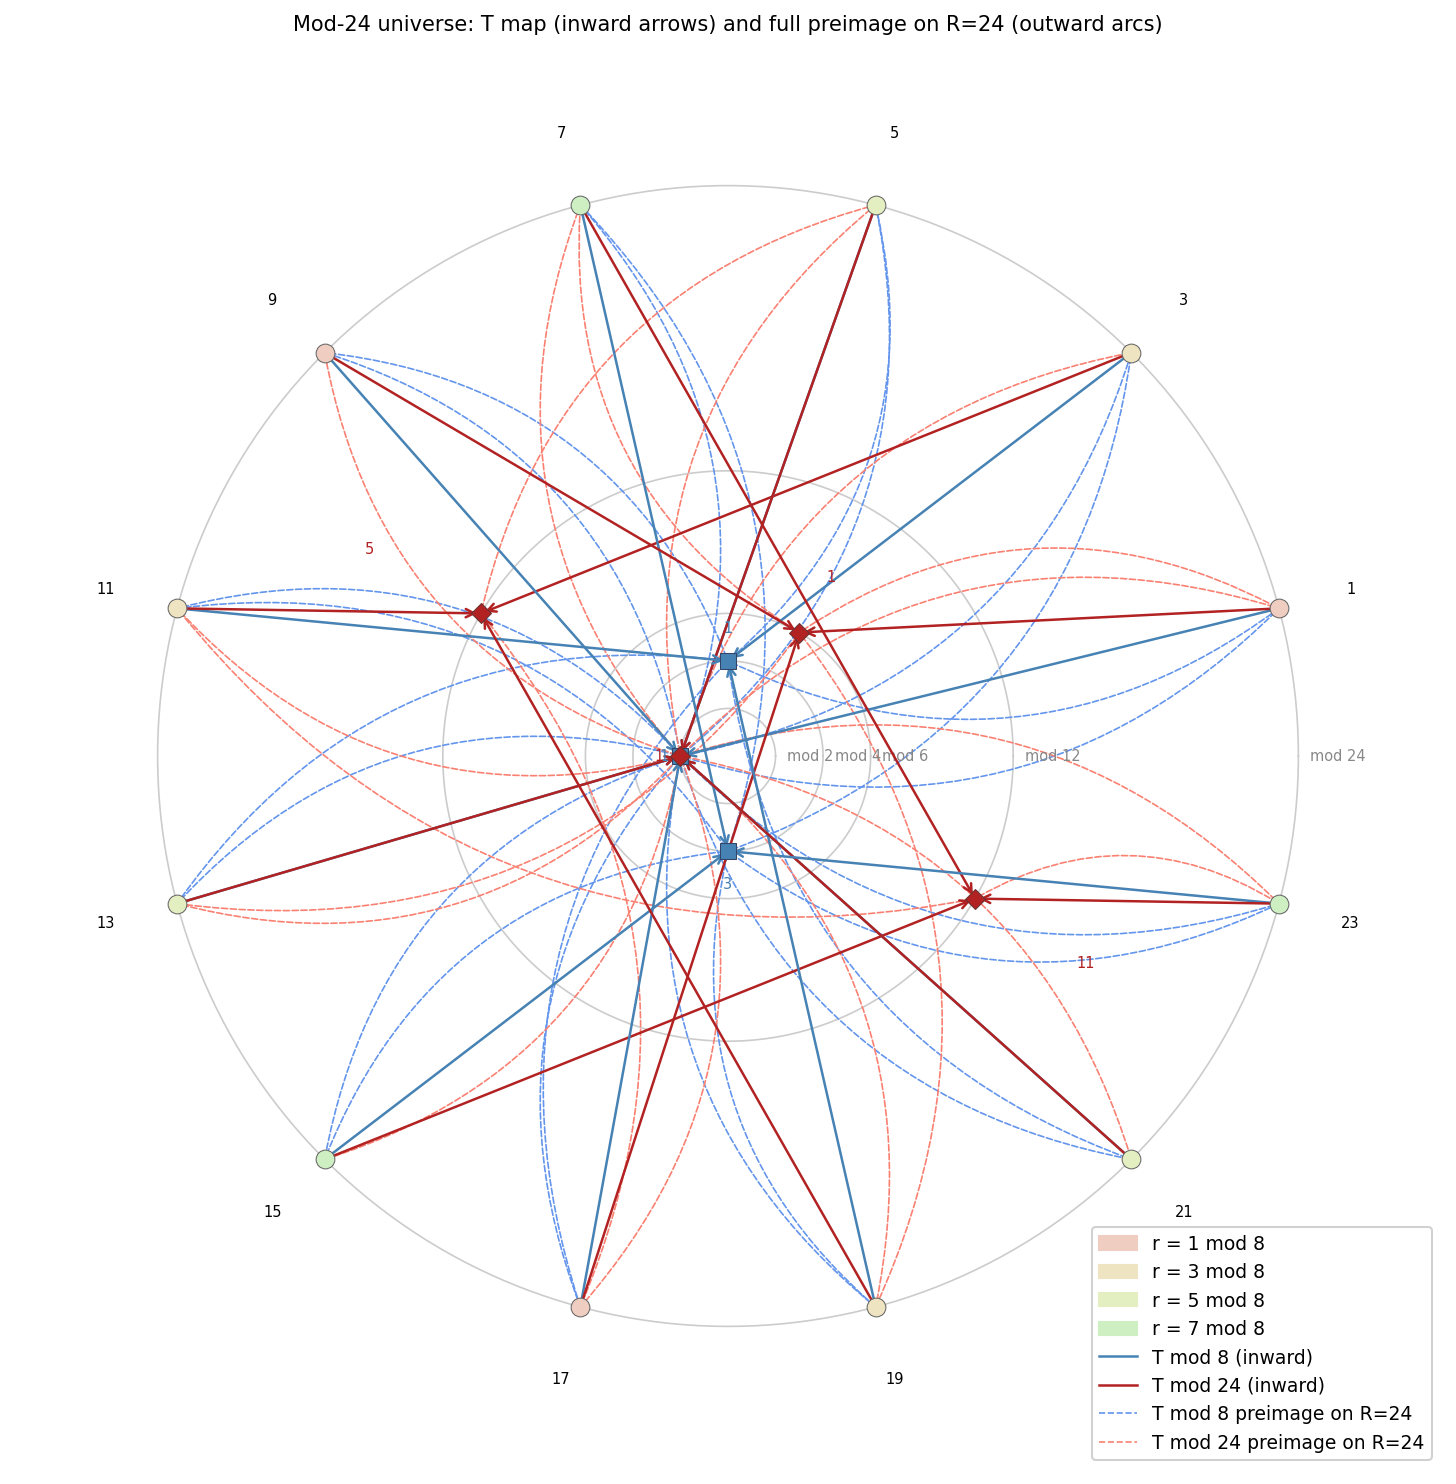
\includegraphics[width=0.85\textwidth]{mod24-universe}
  \caption{The mod-24 universe. Odd input residues $r \in \{1,3,\ldots,23\}$ sit on
    the outer circle ($R=24$) at angle $2\pi r/24$.
    Solid arrows show the image of $S$: blue to the $S \bmod 8$ target on its inner
    circle, red to the $S \bmod 24$ target.
    Dashed arcs show the full arithmetic-progression preimage on $R=24$:
    an output point $kr'+c$ on its circle is connected back to every
    $v \in \{0,\ldots,23\}$ with $v \equiv c \pmod{k}$.}
  \label{fig:mod24-universe}
\end{figure}

\subsection{Mod-8 Reduction}
\label{sec:mod8}

Collapsing the mod-24 table to mod~8 by identifying residue classes with the same
$r \bmod 8$ value yields four odd classes.
The $S \bmod 8$ column is now exact (not a coarsening), and the mod-24 detail is dropped.

\vspace{1em}
\noindent
\footnotesize
\setlength{\tabcolsep}{4pt}
\begin{tabular}{>{\bfseries}r|l|l|l}
\toprule
$r \bmod 8$ & $S(8a+r)$ & $S \bmod 8$ & Note \\
\midrule
\cellcolor{res1}1 & \cellcolor{res1}$6a + 1$ & \cellcolor{res1}$2r''+1$ & \cellcolor{res1}$v_2(3r+1)=2$; all odd outputs \\
\cellcolor{res3}3 & \cellcolor{res3}$12a + 5$ & \cellcolor{res3}$4r''+1$ & \cellcolor{res3}$v_2(3r+1)=1$; outputs $\equiv 1 \pmod{4}$ \\
\cellcolor{res5}5 & \cellcolor{res5}$(3a+2)/2^{v_2(3a+2)}$ & \cellcolor{res5}$2r''+1$ & \cellcolor{res5}$v_2(3r+1)\ge 3$; all odd outputs \\
\cellcolor{res7}7 & \cellcolor{res7}$12a + 11$ & \cellcolor{res7}$4r''+3$ & \cellcolor{res7}$v_2(3r+1)=1$; outputs $\equiv 3 \pmod{4}$ \\
\bottomrule
\end{tabular}
\normalsize

\begin{figure}[h]
  \centering
  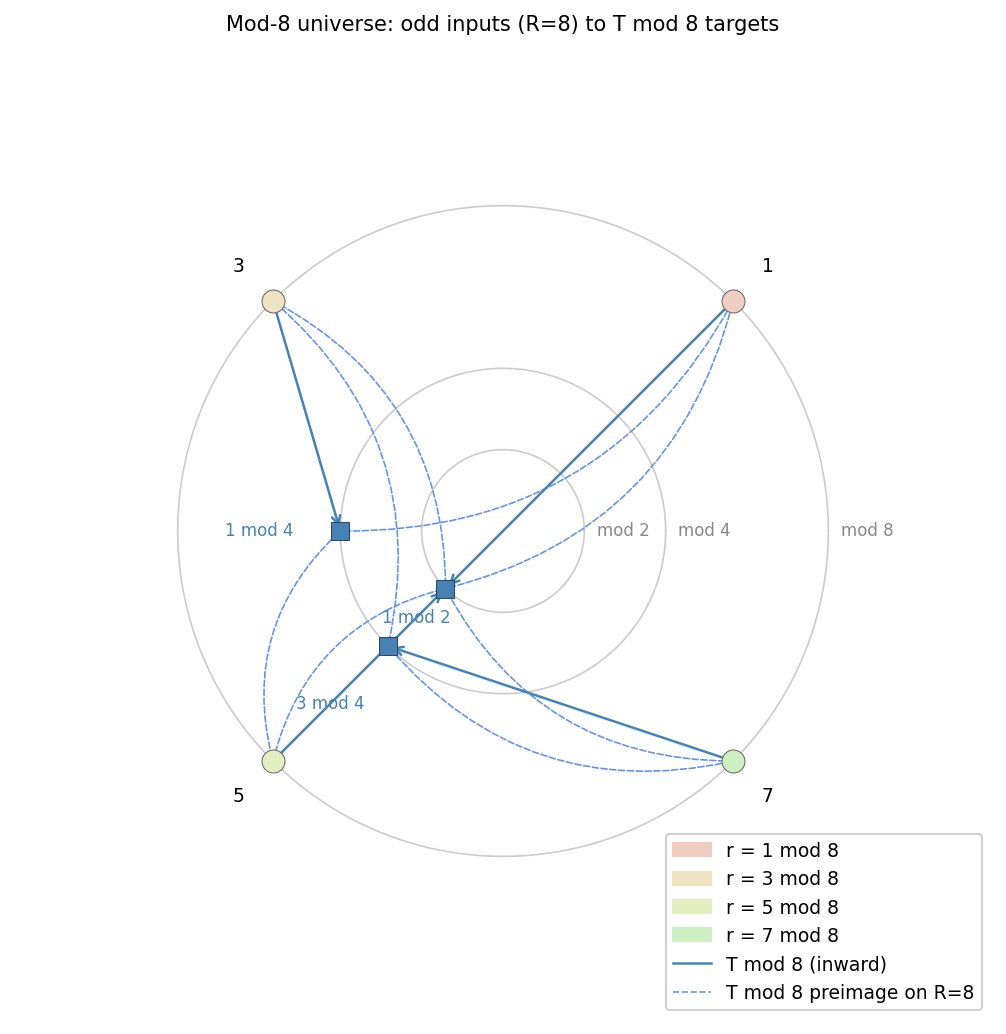
\includegraphics[width=0.75\textwidth]{mod8-universe}
  \caption{The mod-8 universe. The four odd input residues $\{1,3,5,7\}$ sit on the
    outer circle ($R=8$).
    Solid arrows show $S \bmod 8$ targets on inner circles.
    Dashed arcs show the full preimage on $R=8$ of each output class.}
  \label{fig:mod8-universe}
\end{figure}

\subsection{The Mod-8 State Machine}
\label{sec:mod8-state-machine}

\begin{figure}[H]
\centering
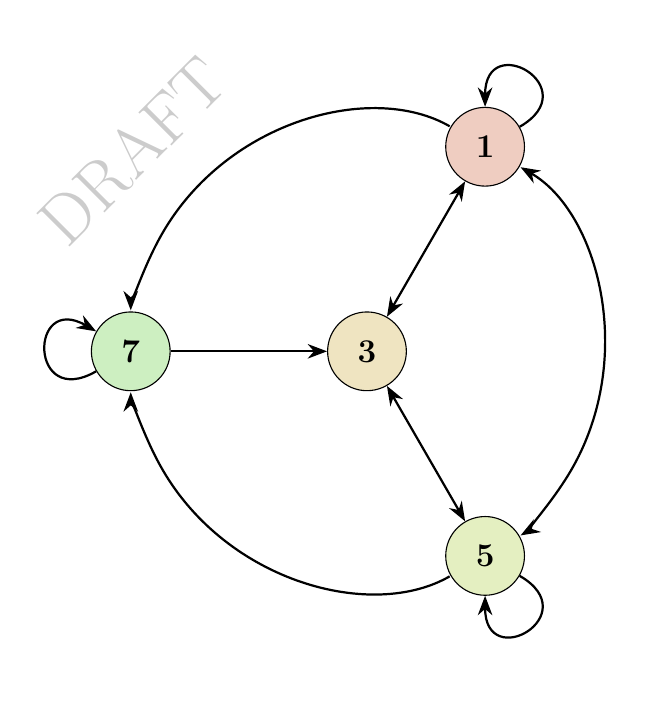
\begin{tikzpicture}[
    every node/.style={circle, draw, minimum size=1.0cm, font=\bfseries\large},
    arr/.style={-{Stealth[length=7pt]}, thick},
  ]
  % 3 at centre; 7, 1, 5 at 180°, 60°, 300° on a circle of radius 3
  \node[fill=res3] (n3) at (0,    0)                        {3};
  \node[fill=res7] (n7) at ({3*cos(180)}, {3*sin(180)})     {7};
  \node[fill=res1] (n1) at ({3*cos(60)},  {3*sin(60)})      {1};
  \node[fill=res5] (n5) at ({3*cos(300)}, {3*sin(300)})     {5};

  % Forward chain 7->3 (one-way, node-to-node auto-clips)
  \draw[arr] (n7) -- (n3);

  % 3 <-> 1 and 3 <-> 5 (bidirectional, auto-clips)
  \draw[{Stealth[length=7pt]}-{Stealth[length=7pt]}, thick] (n3) -- (n1);
  \draw[{Stealth[length=7pt]}-{Stealth[length=7pt]}, thick] (n3) -- (n5);

  % 1 <-> 5 (bidirectional, true circle arc)
  \draw[{Stealth[length=7pt]}-{Stealth[length=7pt]}, thick, shorten >=0.52cm, shorten <=0.52cm]
    ({3*cos(60)},{3*sin(60)}) arc[start angle=60, end angle=-60, radius=3];

  % 1 -> 7 (arc from 60° to 180°, outward above)
  \draw[arr, shorten >=0.52cm, shorten <=0.52cm]
    ({3*cos(60)},{3*sin(60)}) arc[start angle=60, end angle=180, radius=3];

  % 5 -> 7 (arc from 300° to 180°, outward below)
  \draw[arr, shorten >=0.52cm, shorten <=0.52cm]
    ({3*cos(300)},{3*sin(300)}) arc[start angle=300, end angle=180, radius=3];

  % Loops on 7, 1, 5 — pointing outward from circle centre
  \draw[arr] (n7) edge[out=210,in=150,loop,looseness=5] (n7);
  \draw[arr] (n1) edge[out=30, in=90, loop,looseness=5] (n1);
  \draw[arr] (n5) edge[out=330,in=270,loop,looseness=5] (n5);
\end{tikzpicture}
\caption{The mod-8 state machine. The forward chain $7\to3\to\{1,5\}$ funnels
  low-valuation steps toward the two terminal states, shown stacked in the right
  column: $1$ (top, OEE terminal) and $5$ (bottom, OEEE$^+$ terminal).
  Back-links from $1$ (above) and $5$ (below) return to any earlier state.
  Loops on $7$, $1$, $5$: self-transitions are possible.
  Class~$3$ has no loop and no back-links: $3$-steps always output $\equiv 1\pmod{4}$.}
\label{fig:mod8-graph}
\end{figure}

The table below lists every edge of the state machine.
The outbound edge taken from any state is selected exactly by
\[
  S(a) \bmod 8 \;=\; \frac{3a+1}{2^{v_2(3a+1)}} \bmod 8.
\]


\begin{remark}[Threefold symmetry of the mod-8 state machine]
Every structural count in the mod-8 state machine is a multiple of~$3$:
\begin{itemize}
  \item \textbf{In-degree~3}: every state has exactly~3 inbound edges (counting
    self-loops), one from each of its three mod-24 representatives.
  \item \textbf{3 self-loops}: states $7$, $1$, and $5$ each have a self-transition;
    state~$3$ does not.
  \item \textbf{3 bidirectional transitions}: $3\leftrightarrow1$,
    $3\leftrightarrow5$, and $1\leftrightarrow5$.
  \item \textbf{3 unidirectional transitions}: $7\to3$, $1\to7$, and $5\to7$.
\end{itemize}
State~$3$ is the sole exception to self-referentiality: it is a pure funnel,
with no self-loop and no outgoing back-links, receiving from~$\{7,1,5\}$ and
forwarding only to~$\{1,5\}$.
\end{remark}

\subsection{Behaviour of the $7 \bmod 8$ Class}
\label{sec:mod8-seven}

Every odd $n \equiv 7 \pmod{8}$ satisfies $v_2(3n+1) = 1$, so
$S(n) = (3n+1)/2$ and $S(8t+7) = 12t+11$.
The output is $\equiv 3 \pmod{8}$ when $t$ is even and $\equiv 7 \pmod{8}$ when $t$
is odd, so a single step may terminate the run or extend it.
The precise mechanism is the content of Theorem~\ref{thm:7chain} in
Section~\ref{sec:steiner-circuits}: the $7 \bmod 8$ run length is the Steiner
parameter $\alpha - 2$, governed by the Lyapunov metric $\lambda(n) = v_2(n+1)$.

\begin{corollary}[Ping-pong exit]
\label{cor:pingpong}
Let $n = 8t+7$ with $n \equiv 7 \pmod{8}$, and let $\ell = v_2(n+1)-2$ be the
$7^*$ chain length (Theorem~\ref{thm:7chain}). Then
\[
  S^{\ell}(n) \;\equiv\; \begin{cases} 11 \pmod{24} & \text{if } t \text{ is even,} \\
  23 \pmod{24} & \text{if } t \text{ is odd.} \end{cases}
\]
\end{corollary}
\begin{proof}
Each $S$-step on a $7 \bmod 8$ input maps $t \mapsto \frac{3t+1 \cdot \ldots}{2}$
preserving $t$'s parity (since $S(8t+7) = 12t+11$ and $12t+11 = 8(t') + 7$ with
$t' = \frac{3t+1}{2}$ when $t$ is odd, keeping parity through the chain).
The exit value satisfies $S^\ell(n) = 12t'+11$ for $t'$ of the same parity as $t$,
giving $12t'+11 \equiv 11$ or $23 \pmod{24}$ as $t'$ is even or odd.
\end{proof}

\clearpage
% ---------------------------------------------------------------
\section{Sequence Encodings of Collatz Paths}
\label{sec:seqenc}

A Collatz path from an odd integer $a$ to an odd integer $b$ under the natural
map $C$ is a finite sequence of steps, each of which is either an \emph{odd step}
($n \mapsto 3n+1$) or an \emph{even step} ($n \mapsto n/2$).
This section develops a hierarchy of notations for such paths, progressing from
raw binary strings through run-length encodings to the compressed mod-8 circuit
form that underpins the regular expression in Chapter~\ref{sec:regexp}.

\subsection{Mod-2 Notation}

\subsubsection{OE Notation}

The coarsest encoding records only the parity of each $C$-step.
Write $\mathsf{O}$ for an odd step and $\mathsf{E}$ for an even step.
A path that begins at an odd integer and ends just before the next odd integer is
an \emph{OE word}: it consists of exactly one~$\mathsf{O}$ followed by one or more
$\mathsf{E}$s.
For example, the path $3 \to 10 \to 5$ is encoded $\mathsf{OE}$, and
$3 \to 10 \to 5 \to 16 \to 8 \to 4 \to 2 \to 1$ yields $\mathsf{OEEEEE}$.

A longer orbit is obtained by concatenating OE words.
The first few odd iterates of $27$ give, in order:
\[
  27 \;\xrightarrow{\mathsf{OE}}\; 41 \;\xrightarrow{\mathsf{OEE}}\; 31 \;\xrightarrow{\mathsf{OEEE}}\; \cdots
\]
Concatenating the words gives the full OE string for the path.

\subsubsection{OE Compression}

Under Collatz dynamics, every odd step is immediately followed by at least one even
step: $3a+1$ is always even, so $C$ must apply at least one halving after every
$\mathsf{O}$.
The first $\mathsf{E}$ after each $\mathsf{O}$ is therefore redundant ---
its presence is guaranteed by the dynamics.
\emph{Compressed OE notation} drops this redundant $\mathsf{E}$, replacing each
occurrence of $\mathsf{OE}$ with a single $\mathsf{O}$ and leaving all other symbols
unchanged.
For example, $\mathsf{OEOEE}$ compresses to $\mathsf{OOE}$: each $\mathsf{OE}$
becomes $\mathsf{O}$, and the trailing $\mathsf{E}$ is retained.
The surviving $\mathsf{E}$s are the \emph{excess evens} --- the even steps beyond
the mandatory minimum --- and carry the arithmetic weight of the path.

Compressed OE notation coincides with the notation that arises naturally from the
Terras map $T$~\cite{terras1976}, in which the odd step is $(3n+1)/2$ rather than
$3n+1$: that map folds the mandatory halving into the odd step, so its symbol
alphabet records only the excess even halvings.
When this paper writes unexponentiated OE strings, however, we always mean the
\emph{uncompressed} form — explicit $\mathsf{O}$ and $\mathsf{E}$ symbols for
every individual $C$-step.

\subsubsection{Symbol Exponentiation}

Exponential notation operates on the output of compressed OE notation.
A run of $\alpha$ consecutive $\mathsf{O}$s is written $\mathsf{O}^\alpha$,
and a run of $\beta$ consecutive $\mathsf{E}$s is written $\mathsf{E}^\beta$.
Continuing the example, $\mathsf{OOE}$ becomes $\mathsf{O}^2\mathsf{E}^1$,
or simply $\mathsf{O}^2\mathsf{E}$.
A Steiner circuit whose compressed form is $\mathsf{O}^\alpha\mathsf{E}^\beta$
has $\alpha = o$ odd steps and $\beta = e - o$ excess even steps
(total even count $e = \alpha + \beta$), and satisfies $\beta \geq 1$
(the convergence condition $3^\alpha < 2^{\alpha+\beta}$).
The distribution of those $\beta$ excess even steps among the $\alpha$ odd-step
blocks is suppressed in this notation; it is recovered by the mod-8 encoding below.

\subsubsection{Steiner Circuits}
\label{sec:steiner-circuits}

A \emph{Steiner circuit} is a path whose exponential form is
$\mathsf{O}^\alpha\mathsf{E}^\beta$ — that is, all $\alpha$ odd steps precede all
$\beta$ excess even steps in the compressed string.
Such paths have a clean arithmetic characterisation that illuminates why the
exponential notation is natural.

\begin{proposition}[Steiner circuit arithmetic]\label{prop:steiner}
Let $a_0$ be a positive odd integer with $a_0 + 1 = 2^\alpha m$ for some
positive odd integer $m$ and $\alpha \geq 1$.
Then the orbit of $a_0$ under $C$ evolves as follows.
\begin{enumerate}
  \item After $i$ OE pairs ($0 \leq i \leq \alpha$):
    \[
      a_i + 1 \;=\; 3^i \cdot 2^{\alpha - i} \cdot m.
    \]
  \item After $\alpha$ OE pairs, $a_\alpha = 3^\alpha m - 1$, which is even.
  \item The subsequent pure even descent has length $\beta = v_2(3^\alpha m - 1)$,
    terminating at the odd integer
    \[
      b \;=\; \frac{3^\alpha m - 1}{2^\beta}.
    \]
\end{enumerate}
The path from $a_0$ to $b$ has $\alpha$ odd steps and $e = \alpha + \beta$ even
steps in total, and its exponential form is $\mathsf{O}^\alpha\mathsf{E}^\beta$.
\end{proposition}

\begin{proof}
The base case $i=0$ holds by hypothesis.
For the inductive step, suppose $a_i + 1 = 3^i \cdot 2^{\alpha-i} \cdot m$ with
$\alpha - i \geq 1$, so $a_i$ is odd (since $3^i \cdot 2^{\alpha-i} \cdot m$ is even).
One odd step gives
\[
  3a_i + 1 \;=\; 3(a_i + 1) - 2 \;=\; 3^{i+1} \cdot 2^{\alpha-i} \cdot m - 2
  \;=\; 2\bigl(3^{i+1} \cdot 2^{\alpha-i-1} \cdot m - 1\bigr).
\]
The mandatory even step divides by~$2$, giving
$a_{i+1} = 3^{i+1} \cdot 2^{\alpha-i-1} \cdot m - 1$,
so $a_{i+1} + 1 = 3^{i+1} \cdot 2^{\alpha-(i+1)} \cdot m$, completing the induction.

At $i = \alpha$: $a_\alpha + 1 = 3^\alpha m$, which is odd (both factors odd),
so $a_\alpha = 3^\alpha m - 1$ is even and the OE phase ends.
The pure even descent lasts exactly $\beta = v_2(3^\alpha m - 1)$ steps by
definition of the 2-adic valuation, reaching the odd integer $b = (3^\alpha m - 1)/2^\beta$.
The $\alpha$ OE pairs contribute $\alpha$ odd and $\alpha$ even steps;
the final descent contributes $\beta$ more even steps, for $e = \alpha + \beta$ total.
In compressed OE notation the mandatory even steps are suppressed,
leaving $\alpha$ Os followed by $\beta$ Es, i.e.\ $\mathsf{O}^\alpha\mathsf{E}^\beta$.
\end{proof}

\begin{figure}[h]
\centering
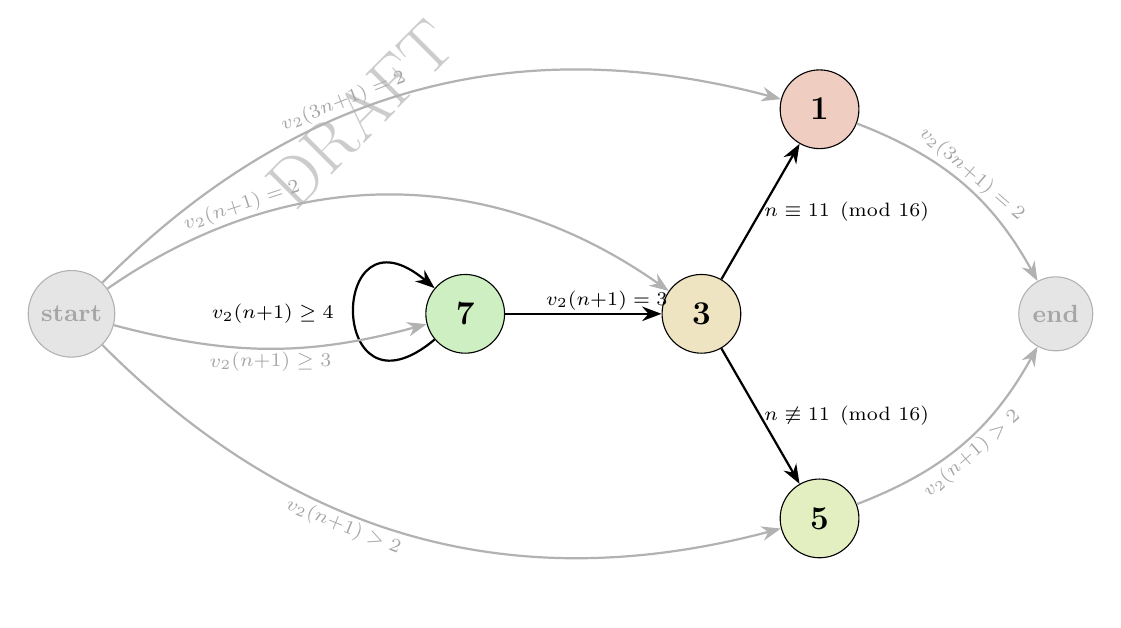
\begin{tikzpicture}[
    st/.style={circle, draw, minimum size=1.0cm, font=\bfseries\large},
    arr/.style={-{Stealth[length=7pt]}, thick},
    grey/.style={circle, draw=gray!60, fill=gray!20, minimum size=0.8cm,
                 font=\small\bfseries, text=gray!70},
    lbl/.style={font=\scriptsize, inner sep=1pt},
    glbl/.style={font=\scriptsize, inner sep=1pt, text=gray!70},
  ]
  % Same geometry as the mod-8 machine: 3 at centre; 7, 1, 5 at 180°, 60°, 300°
  \node[st, fill=res3] (n3) at (0,    0)                        {3};
  \node[st, fill=res7] (n7) at ({3*cos(180)}, {3*sin(180)})     {7};
  \node[st, fill=res1] (n1) at ({3*cos(60)},  {3*sin(60)})      {1};
  \node[st, fill=res5] (n5) at ({3*cos(300)}, {3*sin(300)})     {5};

  % Start node (grey, left of 7) and End node (grey, right)
  \node[grey] (start) at ({8*cos(180)}, {8*sin(180)}) {start};
  \node[grey] (end)   at (4.5, 0)                          {end};

  % Kept edges from the full mod-8 machine
  \draw[arr] (n7) -- node[lbl, above, sloped, pos=0.65] {$v_2(n{+}1)=3$} (n3);
  \draw[arr] (n3) -- node[lbl, right] {$n\equiv 11\pmod{16}$} (n1);
  \draw[arr] (n3) -- node[lbl, right] {$n\not\equiv 11\pmod{16}$} (n5);
  \draw[arr] (n7) edge[out=220,in=140,loop,looseness=7]
    node[lbl, left, xshift=-6pt] {$v_2(n{+}1)\ge4$} (n7);

  % Start -> 7, 3, 1, 5  (arcs route around the 7 node)
  \draw[arr, draw=gray!60, bend right=15] (start)
    to node[glbl, below, sloped, pos=0.5] {$v_2(n{+}1)\ge3$} (n7);
  \draw[arr, draw=gray!60, bend left=30] (start)
    to node[glbl, above, sloped, pos=0.4] {$v_2(3n{+}1)=2$} (n1);
  \draw[arr, draw=gray!60, bend left=35] (start)
    to node[glbl, above, sloped, pos=0.25] {$v_2(n{+}1)=2$} (n3);
  \draw[arr, draw=gray!60, bend right=30] (start)
    to node[glbl, below, sloped, pos=0.4] {$v_2(n{+}1)>2$} (n5);

  % 1 -> end, 5 -> end
  \draw[arr, draw=gray!60, bend left=20] (n1)
    to node[glbl, above, sloped] {$v_2(3n{+}1)=2$} (end);
  \draw[arr, draw=gray!60, bend right=20] (n5)
    to node[glbl, below, sloped] {$v_2(n{+}1)>2$} (end);
\end{tikzpicture}
\caption{Steiner circuit state machine: the mod-8 machine restricted to
  paths of the form $(7^*\,3)^?\,(1|5)$.
  Removed edges: $5\to7$, $1\to7$, $1\to1$, $5\to5$, $5\to3$, $1\to3$, $1\leftrightarrow5$.
  Grey start node connects to every possible circuit entry state;
  grey end node collects the two circuit exit states $1$ and $5$.}
\label{fig:steiner-machine}
\end{figure}

\begin{remark}[Steiner circuit machine as a subgraph of the mod-8 machine]
Figure~\ref{fig:steiner-machine} is obtained from the full mod-8 state machine
(Figure~\ref{fig:mod8-graph}) by deleting seven edges:
$5\to7$, $1\to7$, $1\to1$, $5\to5$, $5\to3$, $1\to3$, and $1\leftrightarrow5$.
The retained edges --- the $7$ self-loop, $7\to3$, $3\to1$, and $3\to5$ --- are
exactly those traversed by Steiner circuits.
This pattern of restricting the mod-8 machine by edge deletion (and occasionally
edge reversal) recurs throughout the paper as a tool for visualising constrained
walk families.
\end{remark}

\begin{remark}[Steiner parameter and the $7 \bmod 8$ run]
\label{rem:steiner-7run}
The parameter $\alpha = v_2(a_0+1)$ in Proposition~\ref{prop:steiner} is the
\emph{precise} count of odd steps in the circuit.
When every odd step is a $7 \bmod 8$ step (i.e.\ the circuit is a pure $7^*$ run
followed by a $3 \bmod 8$ exit), the run length is $\alpha - 2$: the circuit uses
$\alpha - 2$ steps in the $7 \bmod 8$ class and two further steps to complete
the exit transition.
This is the content of Theorem~\ref{thm:7chain} below.
\end{remark}

\begin{lemma}[mod-8 class via $v_2(n+1)$]
\label{lem:mod8-v2}
For any odd integer $n$:
\[
  n \equiv 7 \pmod{8} \;\iff\; v_2(n+1) \ge 3,
  \qquad
  n \equiv 3 \pmod{8} \;\iff\; v_2(n+1) = 2.
\]
\end{lemma}
\begin{proof}
Since $n$ is odd, $n+1$ is even.
The residue $n \bmod 8 \in \{1,3,5,7\}$ determines $n+1 \bmod 8 \in \{2,4,6,0\}$,
and hence $v_2(n+1) \in \{1,2,1,\ge 3\}$ respectively.
\end{proof}

\begin{lemma}[$S$ decrements $v_2(n+1)$]
\label{lem:S-decrement}
If $n \equiv 7 \pmod{8}$ then $v_2(S(n)+1) = v_2(n+1) - 1$.
\end{lemma}
\begin{proof}
Write $n + 1 = 2^s q$ with $q$ odd and $s = v_2(n+1) \ge 3$.
Since $v_2(3n+1) = 1$ we have $S(n) = (3n+1)/2$, so
\[
  S(n) + 1 \;=\; \frac{3n+3}{2} \;=\; \frac{3(n+1)}{2} \;=\; 3 \cdot 2^{s-1} q.
\]
As $3q$ is odd, $v_2(S(n)+1) = s-1$.
The key identity $S(n)+1 = \tfrac{3(n+1)}{2}$ is the fundamental mechanism of
every Steiner circuit: each OE pair replaces one factor of $2$ in $n+1$ by a
factor of $3$, transferring the 2-adic weight downward by exactly one.
\end{proof}

\begin{theorem}[$7^*$ run length and the Steiner parameter]
\label{thm:7chain}
Let $n$ be an odd integer with $n \equiv 7 \pmod{8}$ and $v_2(n+1) = s \ge 3$.
Let $\ell(n)$ be the length of the maximal run of $S$-iterates starting at $n$
that remain $\equiv 7 \pmod{8}$:
\[
  S^j(n) \equiv 7 \pmod{8}\ (0 \le j < \ell), \qquad S^\ell(n) \equiv 3 \pmod{8}.
\]
Then
\[
  \ell(n) \;=\; v_2(n+1) - 2 \;=\; s - 2.
\]
Equivalently, the Steiner parameter of the enclosing circuit satisfies $\alpha = s$,
and the $7^*$ run occupies the first $\alpha - 2$ of the $\alpha$ odd steps.
\end{theorem}
\begin{proof}
By Lemma~\ref{lem:S-decrement}, each $S$-step decrements $v_2(\cdot+1)$ by~1
while the iterate is in the $7 \bmod 8$ class.
After $k$ steps, $v_2(S^k(n)+1) = s-k$.
By Lemma~\ref{lem:mod8-v2}, the iterate remains $\equiv 7 \pmod 8$ iff $s-k \ge 3$,
and exits to $\equiv 3 \pmod 8$ when $s-k = 2$, i.e.\ at $k = s-2$.
\end{proof}

\begin{figure}[h]
\centering
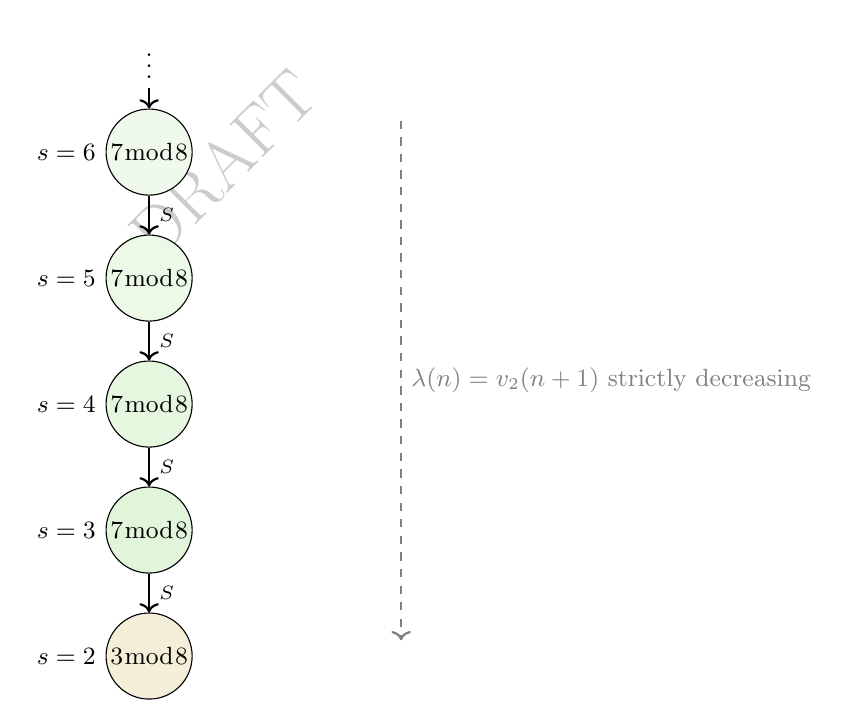
\begin{tikzpicture}[
  every node/.style={font=\small},
  state/.style={circle, draw, minimum size=9mm, inner sep=1pt},
  arr/.style={->, thick},
  lyap/.style={->, thick, dashed, gray},
]
\node[state, fill=res3!60,  label=left:{$s=2$}]  (s2) at (0, 0)   {$3{\bmod}8$};
\node[state, fill=res7!60,  label=left:{$s=3$}]  (s3) at (0, 1.6) {$7{\bmod}8$};
\node[state, fill=res7!50,  label=left:{$s=4$}]  (s4) at (0, 3.2) {$7{\bmod}8$};
\node[state, fill=res7!40,  label=left:{$s=5$}]  (s5) at (0, 4.8) {$7{\bmod}8$};
\node[state, fill=res7!30,  label=left:{$s=6$}]  (s6) at (0, 6.4) {$7{\bmod}8$};
\node[draw=none] (sdots)                          at (0, 7.6) {$\vdots$};
\draw[arr] (s3) -- node[right]{\scriptsize $S$} (s2);
\draw[arr] (s4) -- node[right]{\scriptsize $S$} (s3);
\draw[arr] (s5) -- node[right]{\scriptsize $S$} (s4);
\draw[arr] (s6) -- node[right]{\scriptsize $S$} (s5);
\draw[arr] (sdots) -- (s6);
\draw[lyap] (3.2, 6.8) -- node[right]{\small $\lambda(n)=v_2(n+1)$ strictly decreasing} (3.2, 0.2);
\end{tikzpicture}
\caption{Lyapunov state diagram for $7^*$ runs (Theorem~\ref{thm:7chain}).
States are labelled by $s = v_2(n+1)$; each $S$-step decrements $s$ by~1
(Lemma~\ref{lem:S-decrement}).
The $7 \bmod 8$ class occupies $s \ge 3$; the absorbing state $s=2$ is the
$3 \bmod 8$ exit. Convergence in exactly $s-2$ steps is guaranteed.}
\label{fig:7mod8-lyapunov}
\end{figure}

\begin{remark}[Parity sequences vs.\ concrete sequences]
The notation $\mathsf{O}^\alpha\mathsf{E}^\beta$ describes a \emph{parity sequence}:
it specifies the shape of the path (how many odd and excess-even steps) but not the
concrete starting value.
The free parameter is $m$ in the initial condition $a_0 + 1 = 2^\alpha m$.
To denote a \emph{concrete} Steiner circuit we write $\mathsf{O}^\alpha\mathsf{E}^\beta(m)$,
fixing $m$ and thereby pinning $a_0 = 2^\alpha m - 1$ and all subsequent values uniquely.
\end{remark}

\subsection{Mod-8 Notation}
\label{sec:mod8notation}

\subsubsection{Mod-8 Step Alphabet}
\label{sec:mod8enc}

Moving from the binary alphabet $\{\mathsf{O}, \mathsf{E}\}$ to the four-symbol
odd alphabet $\{1,3,5,7\}$ encodes each $S$-step by the residue class of its
input modulo~8.
From the mod-8 reduction table (Section~\ref{sec:mod8}):

\begin{center}
\begin{tabular}{c|l|c}
\toprule
Symbol & Input class & $v_2(3a+1)$ \\
\midrule
$1$ & $a \equiv 1 \pmod{8}$ & $2$ \\
$3$ & $a \equiv 3 \pmod{8}$ & $1$ \\
$5$ & $a \equiv 5 \pmod{8}$ & $\geq 3$ (varies) \\
$7$ & $a \equiv 7 \pmod{8}$ & $1$ \\
\bottomrule
\end{tabular}
\end{center}

A mod-8 path string is a word over $\{1,3,5,7\}$; for example, $\mathsf{7\,3\,1}$
denotes three consecutive $S$-steps beginning in residue class~$7$, then~$3$, then~$1$.

\subsubsection{Compressed Mod-8 Circuit Form}
\label{sec:compressed}

The mod-8 symbols partition into two groups by their contribution to the step budget:
\emph{high-excess} steps ($5$, contributing $v_2 \geq 3$ even steps)
and \emph{low-excess} steps ($1,3,7$, each contributing $v_2 \leq 2$ even steps).

In a Steiner circuit of parameters $(\alpha, \beta)$ with $\beta \geq 1$,
the circuit terminates with exactly
one terminal symbol:
\begin{itemize}
  \item Symbol $1$ (contributing $v_2 = 2$, so two even steps) when $\beta = 1$
        (one surplus even step: one of the $v_2=2$ drops contributes exactly one
        net surplus after the $S$-step accounting).
  \item Symbol $5$ (contributing $v_2 \geq 3$) when $\beta \geq 2$ (the higher
        valuation absorbs the additional surplus).
\end{itemize}
The remaining $\alpha - 1$ odd steps are filled from the left by $7$-steps
(contributing $v_2 = 1$) and a single $3$-step (contributing $v_2 = 1$) in the
penultimate position (when $\alpha \geq 2$).
This yields the \emph{compressed mod-8 circuit form}:

\begin{equation}
  \label{eq:compressed}
  7^{\alpha-2}\;3^{\alpha-1}\;1^{2-\beta}\;5^{\beta-1}
\end{equation}

where $n^k = \varepsilon$ (the empty string) for $k \leq 0$.
The three mutual exclusions follow immediately:

\begin{center}
\begin{tabular}{c|l|l}
\toprule
$\beta$ & Expanded & Reading \\
\midrule
$1$ & $7^{\alpha-2}\;3^{\alpha-1}\;1^1\;5^0$ & $7^{\alpha-2}\;3^{\alpha-1}\;1$ \\
$2$ & $7^{\alpha-2}\;3^{\alpha-1}\;1^0\;5^1$ & $7^{\alpha-2}\;3^{\alpha-1}\;5$ \\
\bottomrule
\end{tabular}
\end{center}

\begin{remark}[Exponent convention]
The convention $n^k = \varepsilon$ for $k \leq 0$ unifies the boolean
and arithmetic views: $n^{\text{false}}$, $n^0$, $n?$ (regex optional),
and the empty string $\varepsilon$ are all equivalent representations of
``zero occurrences of symbol $n$''.
\end{remark}

\subsubsection{Connection to the Regular Expression}
\label{sec:compreg}

The compressed form~\eqref{eq:compressed} is the bridge to the regular expression
characterisation of Chapter~\ref{sec:regexp}.
Reading off the three syntactic positions:

\begin{center}
\begin{tabular}{c|c|l}
\toprule
Position & Compressed & Regex match \\
\midrule
Leading 7-steps & $7^{\alpha-2}$ & $7^*$ (zero or more) \\
Penultimate 3-step & $3^{\alpha-1}$ & $3?$ (present iff $\alpha \geq 2$) \\
Terminal symbol & $1^{2-\beta}\,5^{\beta-1}$ & $(1\mid 5)$ (exactly one) \\
\bottomrule
\end{tabular}
\end{center}

Each row of the compressed form matches exactly one alternative in the
sub-expression $\bigl((7^*)3?\bigr)?(1\mid 5)$, and a full Collatz path is
a concatenation of such circuits, giving the language
\[
  \bigl((7^*3)?(1\mid 5)\bigr)^*.
\]
This characterisation is stated as Conjecture~\ref{conj:regexp} below;
the proof is deferred to~\cite{paper5}.

\clearpage
% ---------------------------------------------------------------
\section{Graph-Theoretic Foundations}
\label{sec:graphs}

Readers familiar with directed graph theory will find little that is new in this chapter.
The definitions of directed graph, degree, and rooted graph are entirely standard.
Two definitions, however, depart from common usage in ways the rest of this paper relies
on heavily: the distinction between \emph{path} and \emph{walk} (here paths follow edges
and are deterministic; walks oppose them and are not), and the \emph{open/closed} interval
notation for paths.
Readers comfortable with graph theory are encouraged to skim lightly but to read
Definitions~\ref{def:pathwalk} and~\ref{def:openclosed} with care before proceeding.

The default object of study throughout this paper is a \emph{directed graph} (DG),
which may contain cycles.
A \emph{directed acyclic graph} (DAG) is the important special case in which cycles
are absent; its key properties are collected in Definition~\ref{def:dag} and used
where relevant, but they are not assumed to hold by default.
The Collatz graph is a DG: it contains at least the cycle arising from the edge
$(1,1)$ in the odd graph (equivalently, $1 \to 4 \to 2 \to 1$ in the natural graph).
The Collatz conjecture asserts that deleting this single edge --- $(1,1)$ from
$G_S$, or $(1,4)$ from $G_C$ --- leaves a DAG; see
Definition~\ref{def:acyclic}.

\subsection{Directed Graphs: Formal Definitions}

We fix notation that will be used throughout this paper.
All graphs considered here are \emph{directed}; the qualifier is occasionally omitted when
the context is unambiguous.

\begin{definition}[Directed graph]
A \emph{directed graph} is a pair $G = (V, E)$ where
$V$ is a set whose elements are called \emph{nodes} (or \emph{vertices}),
and $E \subseteq V \times V$ is a set whose elements are called \emph{directed edges}.
An edge $(a, b) \in E$ is said to \emph{leave} $a$ and \emph{enter} $b$;
we write $a \to b$ to denote $(a,b) \in E$.
Unless otherwise specified, an edge is represented as the right-open path $[a, b)$:
the source node $a$ is included in the edge's node set and the target node $b$ is not.
\end{definition}

\begin{definition}[In-degree, out-degree, sources and sinks]
The \emph{in-degree} of a node $b \in V$ is the number of edges entering it:
\[
  \deg^-(b) \;=\; \lvert\{b' \in V : b' \to b\}\rvert.
\]
The \emph{out-degree} of a node $a \in V$ is the number of edges leaving it:
\[
  \deg^+(a) \;=\; \lvert\{a' \in V : a \to a'\}\rvert.
\]
A node $a$ with $\deg^-(a) = 0$ is called an \emph{initial node} (or \emph{source}).
A node $b$ with $\deg^+(b) = 0$ is called a \emph{terminal node} (or \emph{sink}).
The conventions $a$ (source) and $b$ (sink) apply at the level of the graph as a whole.
Within local expressions such as edge notation $[a, b)$, $a$ and $b$ denote the
left and right endpoints of that edge and need not be global sources or sinks.
\end{definition}

\begin{definition}[Walk node indexing]
Nodes visited during a walk are written $b_{d,c}$, where $d \ge 0$ is the
\emph{depth} of the node relative to the walk's origin and $c$ is a
\emph{branch label} that identifies which predecessor was chosen at that depth.
The label $c$ is not required to be sequential; it is drawn from an ordered index set
whose specific values are determined by context (for example, a Collatz-derived
metric may yield labels such as $0, 2, 4, \ldots$ or $1, 3, 5, \ldots$).
What is required is only that $c$ uniquely identifies the node among all nodes at
depth $d$ reachable from the walk's origin.
The walk's origin is $b_{0,c_0}$; when the origin is the unique sink of a rooted
tree, it is written $b_{0,0}$.
\end{definition}

\begin{definition}[Path and walk]\label{def:pathwalk}
A \emph{path} of length $k$ in $G$ is a sequence of distinct nodes
$a_0, a_1, \ldots, a_k \in V$ such that $a_{i-1} \to a_i$ for each $1 \le i \le k$,
i.e.\ a path \emph{follows} the direction of edges.
The node $a = a_0$ is the \emph{initial node} and $b = a_k$ is the \emph{terminal node}.
Because edges are followed forward, each successor $a_i$ is uniquely determined by
$a_{i-1}$ whenever $\deg^+(a_{i-1}) = 1$; in a graph where every non-sink node has
out-degree~$1$, a path is \emph{fully determined} by its initial node $a$ and its
length $k$ (or equivalently by $a$ and $b$).

A \emph{walk} of length $k$ in $G$ is a sequence of distinct nodes
$b_{0,c_0}, b_{1,c_1}, \ldots, b_{k,c_k} \in V$ such that
$b_{d,c_d} \to b_{d-1,c_{d-1}}$ for each $1 \le d \le k$,
i.e.\ a walk \emph{opposes} the direction of edges, proceeding back toward the
sources of the graph.
Here $d$ denotes the depth of each node relative to the walk's origin $b_{0,c_0}$,
and $c_d$ is the branch label chosen at depth $d$.
Because edges are opposed, each node $b_{d,c_d}$ is chosen from
$\{p \in V : p \to b_{d-1,c_{d-1}}\}$, which may contain more than one node; a walk is
therefore \emph{non-deterministic} in general.
A walk is fully determined only when a \emph{branch selection procedure} is specified
at every node with in-degree greater than~$1$.

The distinction is definitional and must be maintained throughout: \emph{paths follow
edges and are deterministic; walks oppose edges and require branch selection to be
determined.}

Every path $a_0, a_1, \ldots, a_k$ has a \emph{corresponding walk}
$b_{0,c_0}, b_{1,c_1}, \ldots, b_{k,c_k}$ obtained by traversing the same edges in
reverse: $b_{d,c_d} = a_{k-d}$ for each $0 \le d \le k$.
The walk is the unique branch-selection of the non-deterministic reverse traversal
that recovers exactly the nodes of the path; it is non-deterministic in general
because other branch selections at each $b_{d,c_d}$ may exist.
\end{definition}

\begin{definition}[Open and closed paths; interval notation]\label{def:openclosed}
Let $P = (a_0, a_1, \ldots, a_k)$ be a path with initial node $a = a_0$ and terminal
node $b = a_k$.
\begin{itemize}
  \item A \emph{closed path} $[a, b]$ has node set $\{a_0, a_1, \ldots, a_k\}$;
        both $a$ and $b$ are included.
  \item A \emph{right-open path} $[a, b)$ has node set $\{a_0, a_1, \ldots, a_{k-1}\}$;
        the path traverses all $k$ edges but $b$ is excluded from the node set.
  \item A \emph{left-open path} $(a, b]$ has node set $\{a_1, a_2, \ldots, a_k\}$;
        the path traverses all $k$ edges but $a$ is excluded from the node set.
  \item An \emph{open path} $(a, b)$ has node set $\{a_1, a_2, \ldots, a_{k-1}\}$;
        both endpoints are excluded.
\end{itemize}
In every case the \emph{word of the path} is the label sequence
$\lambda(a_0 \to a_1)\,\lambda(a_1 \to a_2)\cdots\lambda(a_{k-1} \to a_k)$,
which is the same regardless of which endpoints are included in the node set.
A \emph{cycle} $[a, a]$ is a closed path with $a_0 = a_k = a$, $k \ge 1$ edges,
and node set $\{a_0, a_1, \ldots, a_{k-1}\}$ as a set (the closing repetition of $a$
is not a new node); it follows the direction of edges throughout.
Cycles are permitted in a general DG; a graph with no cycles is a DAG
(Definition~\ref{def:dag}), in which every path satisfies $a \ne b$.
\end{definition}

\begin{definition}[Directed acyclic graph]\label{def:dag}
A directed graph $G = (V, E)$ is a \emph{directed acyclic graph} (\emph{DAG})
if it contains no cycle, i.e.\ no closed path $[a, a]$.
Equivalently, the reachability relation on $V$ induced by $E$ is a strict partial order.
A DAG is a special case of a DG; it gains the additional property that every path
reaches a new node at each step.
\end{definition}

\begin{definition}[Rooted directed graph and the unique-successor property]
A directed graph $G = (V, E)$ is \emph{rooted} at $r \in V$ if $r$ is the unique sink
and every node $a \in V$ admits at least one path from $a$ to $r$
(edges point toward $r$, so paths follow them forward to reach $r$).
If in addition $\deg^+(a) = 1$ for every non-sink node $a$, we say $G$ has the
\emph{unique-successor property}; the path from any $a$ to $r$ is then fully
determined, and $G$ is a \emph{directed tree} rooted at $r$.
When the graph is also a DAG, a rooted DG with the unique-successor property
is a \emph{rooted directed tree} in the strict sense (no cycles, one path to root).
\end{definition}

\begin{definition}[Weak connectivity and graph components]
Two nodes $u, v \in V$ are \emph{weakly connected} if they are connected by a path
or walk when all edges are treated as undirected, i.e.\ if there exists a sequence
$u = v_0, v_1, \ldots, v_m = v$ such that for each $1 \le i \le m$ either
$v_{i-1} \to v_i$ or $v_i \to v_{i-1}$ holds in $G$.
Weak connectivity is an equivalence relation on $V$; its equivalence classes are the
\emph{(weakly connected) components} of $G$.
A graph is \emph{weakly connected} if it has exactly one component, i.e.\ every pair
of nodes is weakly connected.

Two nodes $u, v \in V$ are \emph{strongly connected} if there exists both a path from
$u$ to $v$ and a path from $v$ to $u$.
Strong connectivity is likewise an equivalence relation; its classes are the
\emph{strongly connected components} (\emph{SCCs}) of $G$.
In a DAG, every SCC is a single node; non-trivial SCCs (those containing a cycle)
can only arise in a general DG.
\end{definition}

\subsection{Labelled Graphs and Languages}

The graphs arising in this paper carry labels on their edges.

\begin{definition}[Edge-labelled graph]
Let $\Sigma$ be a finite set called the \emph{alphabet}.
An \emph{edge-labelled directed graph} over $\Sigma$ is a triple
$G = (V, E, \lambda)$ where $(V,E)$ is a directed graph and
$\lambda : E \to \Sigma$ assigns a label to each edge.
\end{definition}

\begin{definition}[Word of a path; language of a node]
Given an edge-labelled directed graph $(V,E,\lambda)$ and a path
$a_0, a_1, \ldots, a_k$, the \emph{word of the path} is the concatenation
$\lambda(a_0\to a_1)\,\lambda(a_1\to a_2)\cdots\lambda(a_{k-1}\to a_k) \in \Sigma^*$.
The \emph{language} of a node $a$ is the set of all words produced by paths
starting at $a$:
\[
  \mathcal{L}(a) \;=\;
  \bigl\{\, s \in \Sigma^* \;\big|\; s \text{ is the word of some path starting at } a \,\bigr\}.
\]
\end{definition}

\subsection{The Collatz Graphs}

The maps $C$ and $S$ defined in Definition~\ref{def:maps} are now instantiated as
directed graphs using the framework of the preceding subsections.

\begin{definition}[Natural and odd Collatz graphs]
The \emph{natural Collatz graph} is the directed graph
$G_C = (\mathbb{Z}^+, E_C)$ where $E_C = \{(n, C(n)) : n \in \mathbb{Z}^+\}$.

The \emph{odd Collatz graph} is the directed graph
$G_S = (\mathbb{O}, E_S)$ where $E_S = \{(n, S(n)) : n \in \mathbb{O}\}$.

Both graphs have the unique-successor property: $C$ and $S$ are total maps, so every
node has out-degree exactly~$1$.
$G_C$ contains the cycle $1 \to 4 \to 2 \to 1$; $G_S$ inherits this
as the edge $(1, S(1)) = (1, 1)$, a self-loop at~$1$.
Both graphs are therefore DGs, not DAGs.
\end{definition}

\begin{definition}[Acyclic restrictions and the Collatz conjecture]\label{def:acyclic}
The \emph{acyclic natural graph} is $G_C' = (\mathbb{Z}^+,\; E_C \setminus \{(1,4)\})$,
obtained by deleting the single edge $(1, 4)$ while retaining both nodes.
The \emph{acyclic odd graph} is $G_S' = (\mathbb{O},\; E_S \setminus \{(1,1)\})$,
obtained by deleting the self-loop at~$1$.
In both cases $1$ becomes a sink and the graph is rooted at~$1$.

The \emph{Collatz conjecture} asserts that $G_C'$ and $G_S'$ are DAGs,
i.e.\ that $(1,4)$ is the \emph{only} cycle-forming edge in $G_C$ and that
the self-loop at $1$ is the only cycle in $G_S$.
\end{definition}

\begin{definition}[Collatz paths and walks]
A \emph{natural Collatz path} is a path in $G_C$; an \emph{odd Collatz path}
is a path in $G_S$.
Because both graphs have the unique-successor property, a path in either is fully
determined by its initial node and length.

A \emph{natural Collatz walk} is a walk in $G_C$; an \emph{odd Collatz walk}
is a walk in $G_S$.
Both walks are non-deterministic: positive integers may have multiple predecessors
under $C$, and odd integers may have multiple predecessors under $S$.
A walk in either graph is fully determined only when a branch selection procedure is
specified at every node with in-degree greater than~$1$.

Unless otherwise stated, \emph{Collatz path} and \emph{Collatz walk} refer to the
odd versions $G_S$ and $G_S'$.
\end{definition}

The edge labelling that encodes the arithmetic structure of each step of $S$
is introduced in Section~\ref{sec:regexp}, where the residue alphabet $\{1,3,5,7\}$
is defined and the main language-theoretic conjecture is stated.

\section{Regular Expressions and the Collatz Language}
\label{sec:regexp}

The combinatorial evidence developed in the preceding sections supports the
following central conjecture.

\begin{conjecture}[Regular expression characterisation]
\label{conj:regexp}
Let $n \in \mathbb{O}$ be any odd positive integer and let
$n \to S(n) \to S^2(n) \to \cdots$ be its Syracuse orbit.
Encode each iterate by its residue class mod~8 in the alphabet $\{1,3,5,7\}$.
Then:
\begin{enumerate}
  \item Every maximal Steiner circuit in the orbit matches the regular expression
        $(7^*\,3)?(1\mid 5)$.
  \item The full sequence of Steiner circuits matches $\bigl((7^*\,3)?(1\mid 5)\bigr)^*$.
\end{enumerate}
\end{conjecture}

The infrastructure required for a proof --- the mod-8 step taxonomy,
the Steiner decomposition (Proposition~\ref{prop:steiner}),
the 7-run length theorem (Theorem~\ref{thm:7chain}),
and the mod-24 universe --- is fully developed in the preceding sections.
The proof itself is deferred to~\cite{paper5}.

\section{The 5 Mod~8 Overlay Tree}
\label{sec:overlay}

\emph{Deferred to~\cite{paper5}.}
The 5~mod~8 overlay tree is the sub-DAG of the Collatz graph whose nodes are the
odd integers $\equiv 5 \pmod{8}$ (OEEE$^+$ exit states of Steiner circuits)
and whose edges record the branch structure between consecutive such nodes.
Its combinatorial properties, including the branch-length distribution, are
studied in the companion speculative paper~\cite{paper65}.

\section{Conclusion}
\label{sec:conclusion}

This paper develops the combinatorial infrastructure for a regular-expression
description of Collatz orbits.

\medskip
\noindent\textbf{What is proved.}
\begin{itemize}
  \item The mod-8 step taxonomy (Section~\ref{sec:mod24}): the four residue classes
        $\{1,3,5,7\} \pmod{8}$ correspond exactly to the four OE step types.
  \item The Steiner circuit decomposition (Proposition~\ref{prop:steiner}):
        every Collatz orbit decomposes uniquely into Steiner circuits
        $\mathsf{O}^\alpha\mathsf{E}^\beta$.
  \item The 7-run length theorem (Theorem~\ref{thm:7chain}):
        the length of the maximal $7\bmod 8$ run in a Steiner circuit is
        exactly $v_2(n+1)-2$.
  \item The mod-24 universe (Section~\ref{sec:mod24}):
        mod-24 is the smallest modulus at which the parity prefix of every
        odd residue class is fully determined.
  \item Graph-theoretic foundations (Section~\ref{sec:graphs}):
        definitions and basic properties of the Collatz directed graph $G_S$.
\end{itemize}

\medskip
\noindent\textbf{What is conjectured.}
\begin{itemize}
  \item Conjecture~\ref{conj:regexp}: every Steiner circuit matches $(7^*3)?(1|5)$
        and every orbit matches $((7^*3)?(1|5))^*$.
        Proof deferred to~\cite{paper5}.
\end{itemize}

\medskip
\noindent\textbf{What is deferred.}
\begin{itemize}
  \item The 5~mod~8 overlay tree and branch structure: deferred to~\cite{paper5}
        and the speculative paper~\cite{paper65}.
  \item Cycle-theoretic and convergence results: deferred to~\cite{paper8}.
\end{itemize}

% ---------------------------------------------------------------
\begin{thebibliography}{9}

\bibitem{terras1976}
R.~Terras,
A stopping time problem on the positive integers,
\emph{Acta Arithmetica} \textbf{30} (1976), 241--252.

\bibitem{paper5}
J.~Seymour,
\emph{A Toolkit for Collatz Path Analysis} (Paper~5),
in preparation, 2026.

\bibitem{paper8}
J.~Seymour,
\emph{Applications of the mod-8 regular expression language toolbox to the Collatz conjecture} (Paper~8),
in preparation, 2026.

\bibitem{paper65}
J.~Seymour,
\emph{The $\frac{1}{3}(3/4)^k$ Distribution of Steiner Circuit Branch Lengths} (Speculative Results, Paper~65),
in preparation, 2026.

\end{thebibliography}

\end{document}
